%%%%%%%%%%%%%%%%%%%%%%%%%%%%%%%%%%%%%%%%%
% Thin Sectioned Essay
% LaTeX Template
% Version 1.0 (3/8/13)
%
% This template has been downloaded from:
% http://www.LaTeXTemplates.com
%
% Original Author:
% Nicolas Diaz (nsdiaz@uc.cl) with extensive modifications by:
% Vel (vel@latextemplates.com)
%
% License:
% CC BY-NC-SA 3.0 (http://creativecommons.org/licenses/by-nc-sa/3.0/)
%
%%%%%%%%%%%%%%%%%%%%%%%%%%%%%%%%%%%%%%%%%

%----------------------------------------------------------------------------------------
%	PACKAGES AND OTHER DOCUMENT CONFIGURATIONS
%----------------------------------------------------------------------------------------

\documentclass[a4paper, 11pt]{article} % Font size (can be 10pt, 11pt or 12pt) and paper size (remove a4paper for US letter paper)

\usepackage[protrusion=true,expansion=true]{microtype} % Better typography
\usepackage{graphicx} % Required for including pictures
\graphicspath{{images/}}
\usepackage{wrapfig} % Allows in-line images

\usepackage{amsmath} 
\usepackage{mathpazo} % Use the Palatino font
\usepackage[T1]{fontenc} % Required for accented characters
\linespread{1.05} % Change line spacing here, Palatino benefits from a slight increase by default

\makeatletter
\renewcommand\@biblabel[1]{\textbf{#1.}} % Change the square brackets for each bibliography item from '[1]' to '1.'
\renewcommand{\@listI}{\itemsep=0pt} % Reduce the space between items in the itemize and enumerate environments and the bibliography

\renewcommand{\maketitle}{ % Customize the title - do not edit title and author name here, see the TITLE block below
\begin{flushright} % Right align
{\LARGE\@title} % Increase the font size of the title

\vspace{50pt} % Some vertical space between the title and author name

{\large\@author} % Author name
\\\@date % Date

\vspace{40pt} % Some vertical space between the author block and abstract
\end{flushright}
}

%----------------------------------------------------------------------------------------
%	TITLE
%----------------------------------------------------------------------------------------

\title{\textbf{High Frequency Transformer Design Report}\\ % Title
Work Package 4} % Subtitle

\author{\textsc{Ozan Keysan} % Author
\\{\textit{University of Edinburgh}}} % Institution

\date{\today} % Date

%----------------------------------------------------------------------------------------

\begin{document}

\maketitle % Print the title section

%----------------------------------------------------------------------------------------
%	ABSTRACT AND KEYWORDS
%----------------------------------------------------------------------------------------

%\renewcommand{\abstractname}{Summary} % Uncomment to change the name of the abstract to something else

\begin{abstract}
This report presents the material options for the core of the medium frequency transformer that is being investigated within the Work Package 4 of the ``Next Generation HVDC Network for the OffshoreRenewable Energy Indusrty'' project. 
\end{abstract}

\hspace*{3,6mm}\textit{Keywords:} medium frequency transformer, HVDC transmission, core losses, HV transformer % Keywords

\vspace{30pt} % Some vertical space between the abstract and first section

%----------------------------------------------------------------------------------------
%	ESSAY BODY
%----------------------------------------------------------------------------------------

\section*{Introduction}


\section*{Core Materials}

Although, various types of electrical steel laminations are commonly used in power transformers. As the operating frequency is increased, there are more options available:

\subsection*{Amorphous Materials}

Amorphous cores are typically made of Metglas (metalic glass alloy), which is a thin non-crystalline amorphous metal alloy of iron, boron, silicon and phosphorus. The material has a much higher resistivity in electrical steel which results in a low eddy losses. Furthermore, the hysteresis losses are lower, thus, no-load losses in a transformer with amorphous core will be much lower compared to one with electrical steel. However, amorphous materials usually have lower saturation flux density compared to conventional iron-silicon electrical steel.

Some manufacturers of amorphous transformer cores can be listed as:

\begin{itemize}
  \item Hitachi Metals (Powerlite)
  \item Vacuumschmelze (Vitrovac)
  \item Metglas
  \item Vijai Electricals
\end{itemize}

Amorphous materials are superior to electrical steel laminations. However, nano-crystalline materials are superior to amorphous materials, with their lower cost, higher flux densities \cite{vitroperm_vitrovac}. Nano-crystalline materials will be discussed in the next section. The specifications of amorphous and nano-crystalline materials are compared in Table~\ref{vitropermvitrovac}. The only  application that a amorphous material can be more advantageous is the  high-frequency single-ended forward converter topologies. For other topologies, the nano-crystalline materials are though to be more suitable.

\begin{table}[]
\begin{center}
\begin{tabular}{lcc}
 & Amorphous & Nano-crystalline \\ 
 & (Vitrovac) & (Vitroperm) \\
\hline
Saturation Flux Density & 0.8 T & 1.2 T \\
Losses (f= 20 kHz, B=0.2 T) & 2 W/kg & 1.4 W/kg \\
Max. Operating temperature & $110\,^{\circ}\mathrm{C}$ & $120\,^{\circ}\mathrm{C}$ \\
Curie temperature & $365\,^{\circ}\mathrm{C}$ & $600\,^{\circ}\mathrm{C}$ \\
\hline
\end{tabular} 
\end{center}
\caption{Comparison of amorphous (Vitrovac) and nano-crystalline (Vitroperm) materials \cite{vitroperm_vitrovac}.}
\label{vitropermvitrovac}
\end{table}

\subsection*{Nano-crystalline}

Nano-crystalline is a fairly new material that consists of approximately 80\% of iron with the remaining is mixture of silicon, boron, carbon, nickel and other materials. This is a special type of amorphous material, which has superior magnetic characteristics, such as lower core loss and high permeability. Other specifications can be listed as \cite{Magnetics}:

\begin{itemize}
  \item Up to 50 \% permeability than 80\% nickel material (e.g. Supermalloy).
  \item High saturation flux density (1.2-1.5 T).
  \item High operating temperature up to $130\,^{\circ}\mathrm{C}$.
  \item Minimal change of magnetic characteristics with temperature.
  \item 17 \% lighter than Nickel with a density of 7.3 $\mathrm{g/cm^3}$.
  \item Stacking density up to 90 \% can be achieved.
\end{itemize}


Some main manufacturers of nano-crystalline materials can be listed as:

\begin{itemize}
  \item MK Magnetics
  \item Vacuumschmelze
  \item Hill-Tech
\end{itemize}

In this section, different types of nano-crystalline materials will be compared. 
Vacuumschmelze manufactures the following soft magnetic nano-crystalline materials:


\subsubsection*{VitroPerm}


Nanocrystalline VITROPERM alloys are based on Fe with Si and B with Nb and Cu additives \cite{vitroterm_manual}. VITROPERM nano-crystalline alloys are optimized to combine highest permeability and lowest coercive field strength. The combination of very thin tapes and the relatively high electrical resistance (1.1-1.2~$\mu \Omega m$) to ensure minimal eddy current losses and an outstanding frequency vs. permeability behaviour. Along with saturation flux density of 1.2 T and wide operational temperature range, these features combine to make VITROPERM  superior in many aspects to commonly used ferrite and amorphous materials. Magnetization curves and B-H characteristics of Vitroperm material are presented in 

\begin{figure}[]
  \centering
    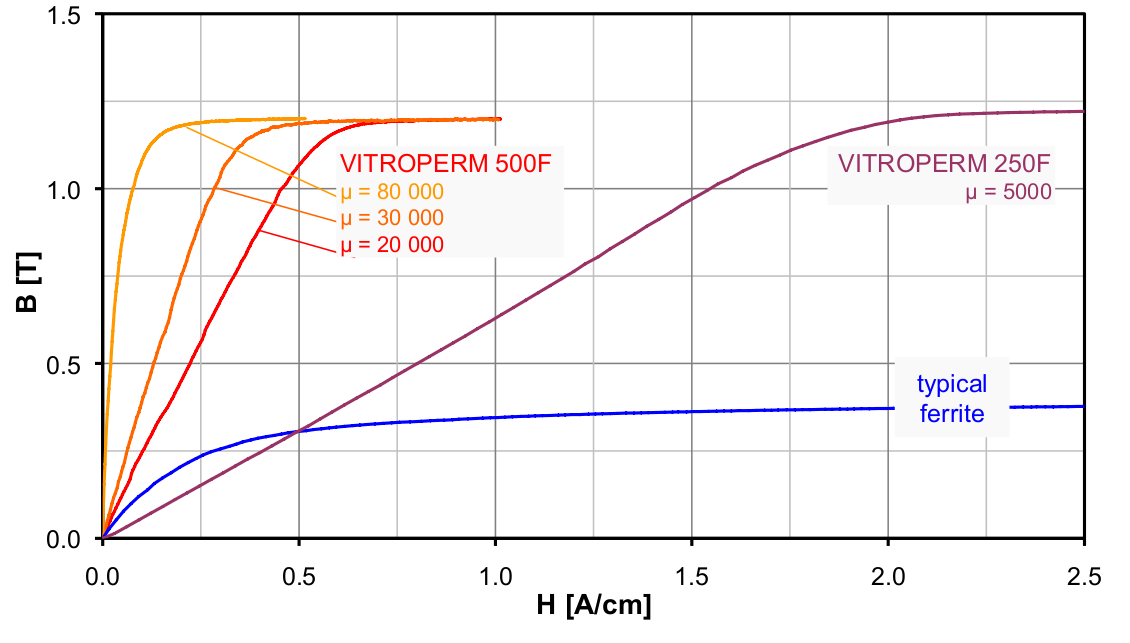
\includegraphics[scale=0.3]{vitroperm_magnetization}
    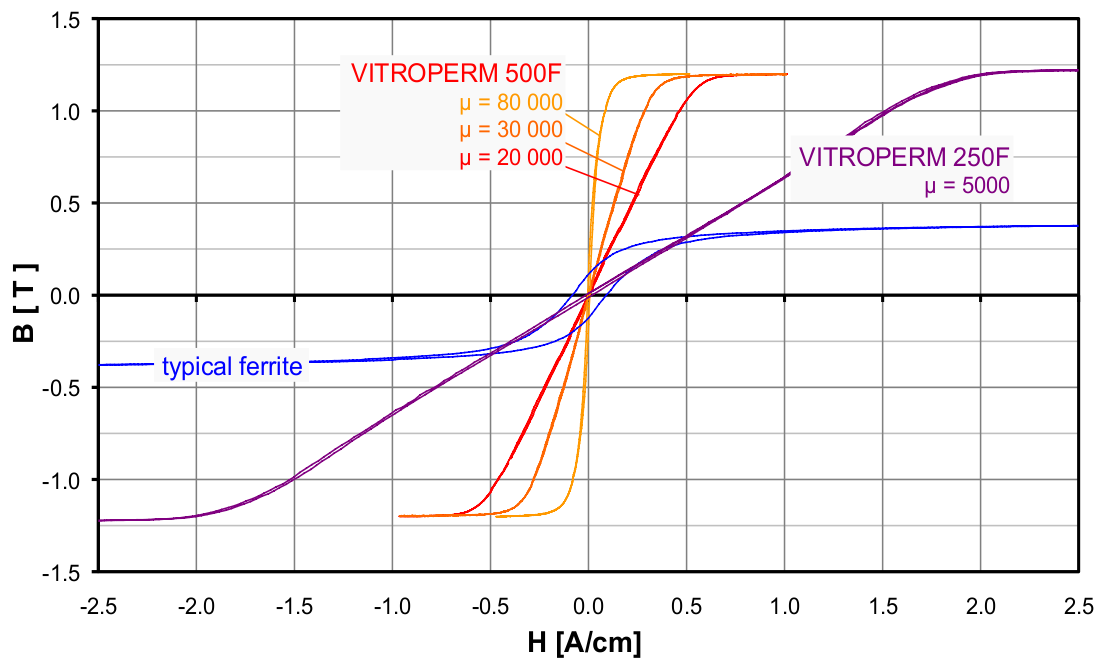
\includegraphics[scale=0.3]{vitroterm_hysteresis}
    \caption{Magnetisation curve and B-H characteristics of Vitroperm \cite{vitroterm_manual}.}
  \label{vitroterm_BH}
\end{figure}

Vitroperm has a wide range material options with different permeability scale as as shown in Fig.~\ref{vitroterm_permeability}. 
The permeability of Vitroperm 500F is significantly higher than ferrite as shown in Fig.~\ref{vitroperm500_250_permeability}.

\begin{figure}[]
  \centering
    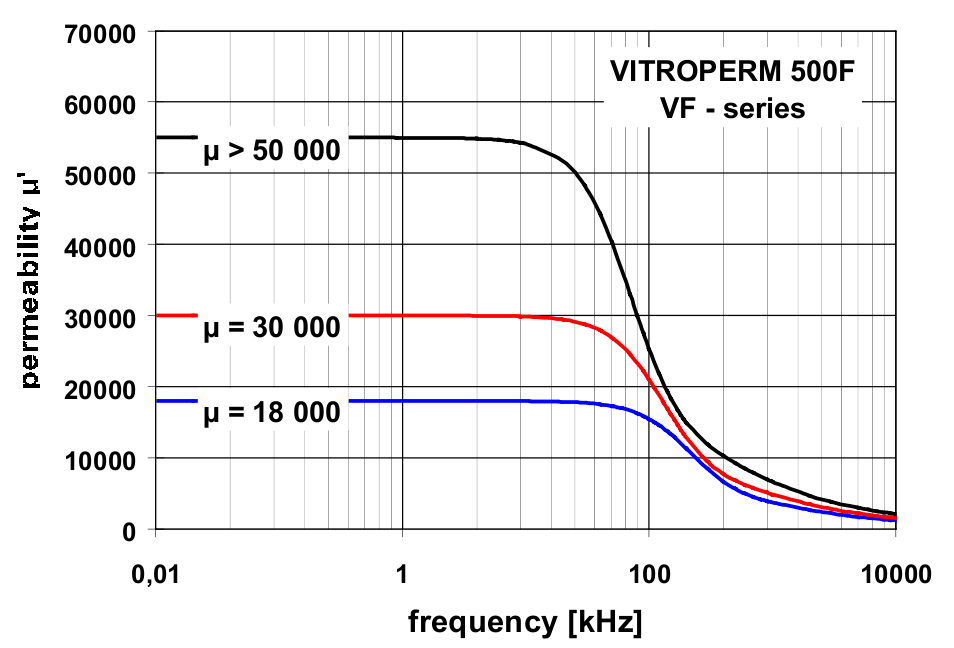
\includegraphics[scale=0.3]{vitroterm_permeability}
  \caption{Permeability change of different Vitroperm materials with frequency \cite{vitroterm_toroidal}.}
  \label{vitroterm_permeability}
\end{figure}

\begin{figure}[]
  \centering
    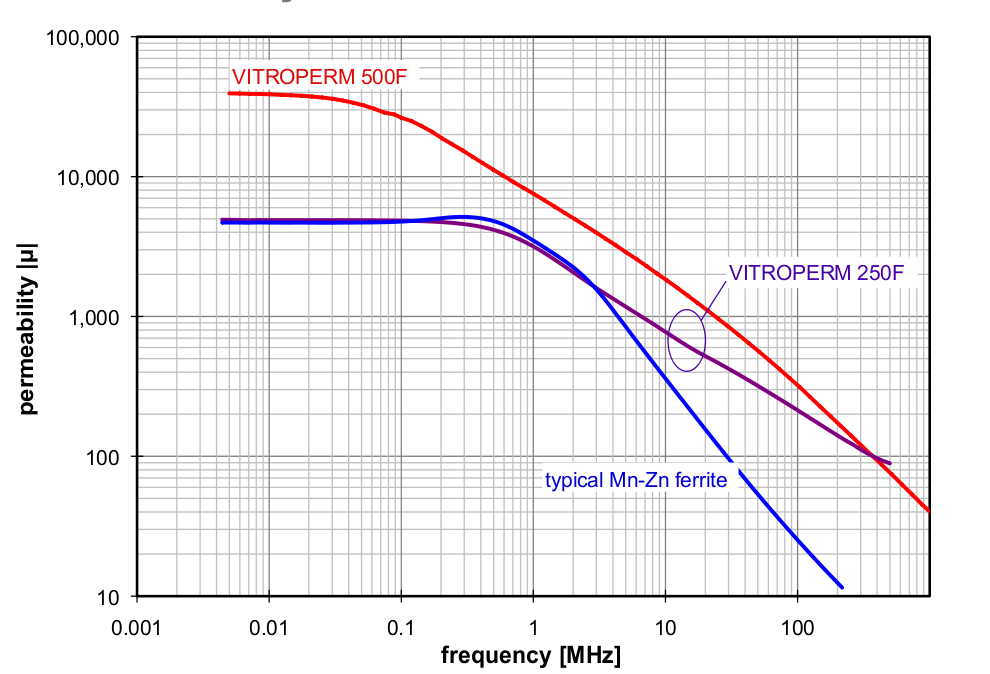
\includegraphics[scale=0.3]{vitroperm500_250_permeability}
  \caption{Permeability change of Vitroperm 250F($\mu = 5000$), Vitroperm 500F($\mu = 40000$) and ferrite($\mu = 5000$) with frequency. \cite{vitroterm_manual}.}
  \label{vitroperm500_250_permeability}
\end{figure}


Vitroperm has also a high operating temperature compared to ferrite. The Curie temperature of Vitroperm alloys are $600\,^{\circ}\mathrm{C}$. Furthermore, the saturation flux density only reduces by 10\% at $120\,^{\circ}\mathrm{C}$, which allows the core can be overloaded for short-amount of periods up to $180-200 \,^{\circ}\mathrm{C}$. The variation of permeability with temperature for Vitroperm is presented in Fig.~\ref{temp_vs_saturation}.

\begin{figure}[]
  \centering
    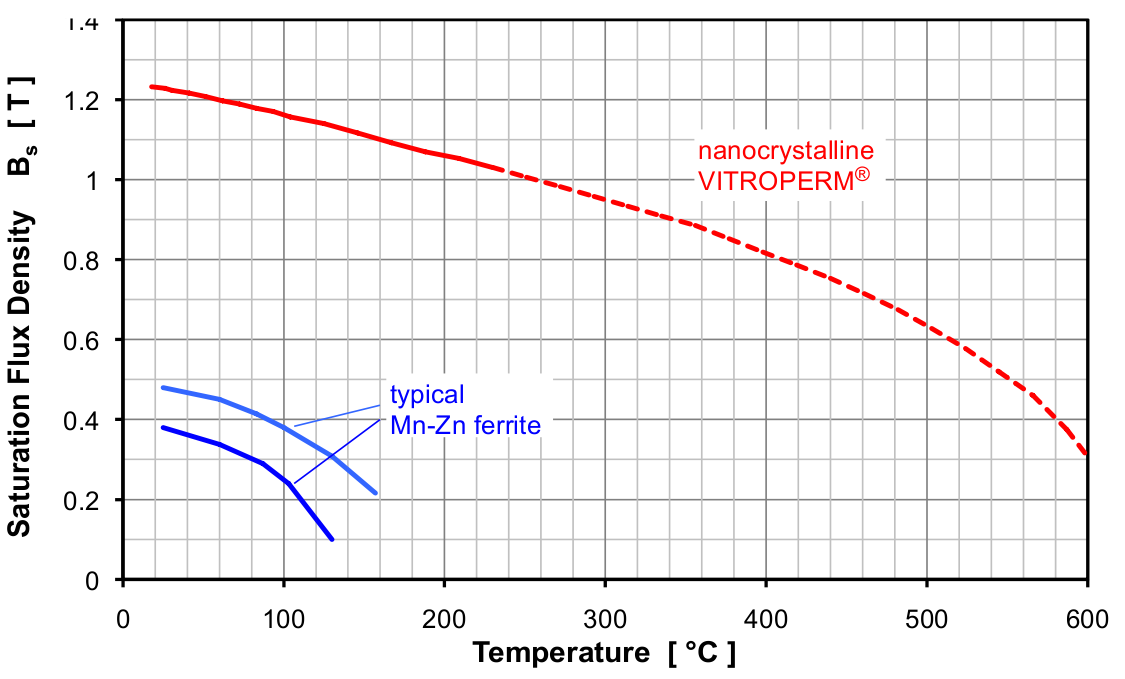
\includegraphics[scale=0.3]{temp_vs_saturation}
  \caption{Saturation flux density variation of Vitroperm with temperature.}
  \label{temp_vs_saturation}
\end{figure}

%Density: 7.35 g/cm3

## Material Comparison \cite{Villar2010}

figure: material_table_villar_2010  (referanslari mendeleyden eklendi: \cite{Heinemann2002} \cite{Steiner2007} \cite{Pavlovsky2005} \cite{Morren2002} \cite{Prasai2007})
Table -1- MF power transformer designs and physical prototypes found in the literature.

It can be seen from the table that nano-crystalline and amorphous materials are the most suggested materials for medium frequency transformers that work between 1 kHz and 25 kHz.


Silicon-Steel: It is a popular choice in line frequency power transformers for its low cost and high-saturation magnetic induction. However, core losses of silicon-steel is high, which makes them unsuitable for medium frequency transformers.

Amorphous and Nanocrystalline: 
These materials have relatively high saturation point (1.2 - 1.56 T), and the reduced losses make them a suitable core material for applications in the 1-25 kHz range. Furthermore, the performance of these materials does not change significantly with temperature, thus it would be possible to choose a higher operating temperature \cite{Villar2010}. 

Ferrites:
Ferrites have a low-loss density in high-frequencies, which makes them a suitable material for high-frequency applications such as RF-filters and chokes. However, they have saturation flux density around 0.5 T, which increases the core volume in high power applications.


The hysteresis losses and the core loss of different materials are compared in \cite{Villar2010}

hysteresis-losses.png \cite{Villar2010}
core-loss.png

\subsection{AC Winding Losses}

The high frequency excitation has two main effects in the transformer windings:
\begin{itemize}
  \item Skin Effect: In AC excitation the current itself generates an opposing magnetic field and current, which reduce the net current density inside the conductor. The total current will stay same, but the distribution will be higher across the circumference of the conductor.
  \item Proximity Effect is the interaction between two adjacent conductors that alters the current distribution in the conductor. Same principles(e.g. proximity, frequency) apply in the proximity affect.
\end{itemize}

Foil conductors are favoured in primary windings of high frequency transformers as the conductor thickness can be reduced while achieving a high cross-section area.

Dowell calculated eddy losses in transformer windings in \cite{Dowell1966}. A detailed explanation of these one dimensional Maxwell equations can be found in \cite{Villar2010}. Referring those equations, the DC resistance of a foil winding can be expressed as:

\begin{equation}
  R_{dc} = \rho \frac{L_{mean}}{t_w h_w} N_{turns}
\end{equation}

where $L_{mean}$ is the mean turn length of the coil, $t_w$ is the thickness, $h_w$ is the height, $\rho$ is the resistivity of copper.

The AC resistance is more complicated and depends on the ratio of the wire thickness to skin depth ($\delta$):

\begin{equation}
  R_{ac}=\rho \frac{L_{mean}}{h_w \delta} N_{turns} \left[\varsigma_1 + \frac{2}{3} (N_{turns}^2-1)\varsigma_2\right]
\end{equation}
where:

\begin{equation}
  \varsigma_1 = \dfrac{sinh(2\Delta)+sin(2\Delta)}{cosh(2\Delta)-cos(2\Delta)} \quad
  \varsigma_2 = \dfrac{sinh(\Delta)-sin(\Delta)}{cosh(\Delta)+cos(\Delta)} \quad  
  \Delta = \dfrac{t_w}{\delta}
\end{equation}

Thus, the important factor is the penetration factor (i.e the ratio of conductor thickness to skin depth, $\Delta$). The ratio of AC resistance to DC resistance is called Dowell's resistance factor ($F_r$). The resistance factor as a function of penetration ratio for a 2 mm thick foil wire is presented in Fig.~\ref{resistance_factor}. For example, at 1 kHz the skin depth is 2.1 mm (the penetration ratio is approximately 1), the resistance factor is 2.7 for a layer number of 4. Thus the resistive losses will be 2.7 times more compared to DC conduction.

\begin{figure}[]
  \centering
    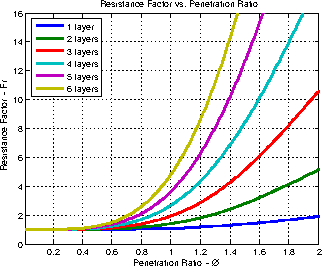
\includegraphics[scale=1.25]{resistance_factor}
  \caption{Resistance factor for a function of penetration ratio (for 2 mm thick foil conductor) \cite{Villar2010}.}
  \label{resistance_factor}
\end{figure}


!! Secondary winding factorunu karsilastir
\cite{Sullivan2003,Ferreira1994} makalelerini oku

\section{Secondary-Winding}
kablo katalogu
http://dielectricsciences.thomasnet.com/viewitems/all-categories/wire-cable-2

%----------------------------------------------------------------------------------------
%	BIBLIOGRAPHY
%----------------------------------------------------------------------------------------

\bibliographystyle{unsrt}

\bibliography{../refler/NAREC}

%----------------------------------------------------------------------------------------

\end{document}